% Generado desde docs/INFORME.md. Editar libremente.

\begin{landscape}
\section{8. Separación privada y agregaciones GraphQL}
La pantalla del pedido de Javiera muestra el pedido, sus pagos y los productos que compró, y esos datos viven en tres servicios distintos. Para que el navegador no tenga que llamarlos uno por uno (ni pueda hacerlo), existe un GraphQL Gateway privado que los junta en una sola consulta. Esta sección muestra cómo está construido, qué puede ver cada rol, qué límites evitan abusos y la evidencia de que funciona desde la pantalla real.

\subsection{Mapa de clasificación}
\vspace{0.6em}
{\scriptsize
\setlength{\LTpre}{0pt}\setlength{\LTpost}{0pt}
\setlength{\tabcolsep}{3pt}\renewcommand{\arraystretch}{1.15}
\begin{longtable}{|>{\raggedright\arraybackslash}p{\dimexpr 0.1115\linewidth-2\tabcolsep\relax}|>{\raggedright\arraybackslash}p{\dimexpr 0.1297\linewidth-2\tabcolsep\relax}|>{\raggedright\arraybackslash}p{\dimexpr 0.1674\linewidth-2\tabcolsep\relax}|>{\raggedright\arraybackslash}p{\dimexpr 0.0887\linewidth-2\tabcolsep\relax}|>{\raggedright\arraybackslash}p{\dimexpr 0.0918\linewidth-2\tabcolsep\relax}|>{\raggedright\arraybackslash}p{\dimexpr 0.1413\linewidth-2\tabcolsep\relax}|>{\raggedright\arraybackslash}p{\dimexpr 0.2696\linewidth-2\tabcolsep\relax}|}
\hline
\textbf{Servicio} & \textbf{Naturaleza} & \textbf{Responsabilidad} & \textbf{Datos propios} & \textbf{Contrato} & \textbf{Dependencias} & \textbf{Justificación de la separación} \\ \hline
\endfirsthead
\hline
\textbf{Servicio} & \textbf{Naturaleza} & \textbf{Responsabilidad} & \textbf{Datos propios} & \textbf{Contrato} & \textbf{Dependencias} & \textbf{Justificación de la separación} \\ \hline
\endhead
inventario & Transaccional & Catálogo, precio, stock & items, reservas & REST & — & Es la fuente de verdad del precio; lo lee la tienda entera \\ \hline
clientes & Transaccional & Ficha personal & clientes & REST & Auth & Aísla los datos personales \\ \hline
pedidos & Transaccional & Ciclo de vida, venta, boleta, reporte & pedidos & REST + eventos STOMP & inventario, clientes, pagos & Núcleo del negocio \\ \hline
pagos & Transaccional / integración & Proveedor externo, dinero & pagos & REST + webhook firmado & pedidos, pasarela & Aísla al proveedor y el riesgo financiero \\ \hline
Auth Service & Seguridad & Credenciales y sesiones & cuentas & REST interno & — & Las credenciales no se mezclan con datos de negocio \\ \hline
GraphQL Gateway & Agregación & Composición de lecturas & Ninguno & GraphQL & pedidos, pagos, inventario, clientes & Las pantallas de detalle y reportes necesitan datos de varios servicios en una sola llamada \\ \hline
notificador & Asíncrono & Correos y avisos & Ninguno & STOMP & ActiveMQ & No bloquea el pago \\ \hline
Analítica / alta demanda & — & No se separan & — & — & — & ADR 0001: la carga no lo justifica \\ \hline
\end{longtable}
}
\end{landscape}

Todos son privados (red \texttt{internal}). Vault, Mongo y ActiveMQ tampoco tienen puertos publicados.


\subsection{Schema}

\begin{codigo}
type Query \{\par
\hspace*{2\ttw}resumenPedido(\allowbreak{}id:\allowbreak{} ID!):\allowbreak{} ResumenPedido\par
\hspace*{2\ttw}misPedidos(\allowbreak{}primeros:\allowbreak{} Int =\allowbreak{} 10,\allowbreak{} despuesDe:\allowbreak{} String):\allowbreak{} PaginaPedidos!\par
\hspace*{2\ttw}reporteVentas(\allowbreak{}desde:\allowbreak{} String!,\allowbreak{} hasta:\allowbreak{} String!):\allowbreak{} ReporteVentas\par
\}\par
type ResumenPedido \{ pedido:\allowbreak{} Pedido!  pagos:\allowbreak{} [\allowbreak{}Pago!]  cliente:\allowbreak{} FichaCliente \}\par
type Pedido \{ id:\allowbreak{} ID! clienteId:\allowbreak{} ID! estado:\allowbreak{} String! estadoTexto:\allowbreak{} String! modoEntrega:\allowbreak{} String!\par
\hspace*{14\ttw}direccion:\allowbreak{} String nota:\allowbreak{} String chofer:\allowbreak{} String total:\allowbreak{} Int! creadoEn:\allowbreak{} String!\par
\hspace*{14\ttw}lineas:\allowbreak{} [\allowbreak{}Linea!]! boleta:\allowbreak{} Boleta anulacion:\allowbreak{} Anulacion historial:\allowbreak{} [\allowbreak{}Paso!]! \}\par
type Linea \{ descripcion:\allowbreak{} String! cantidad:\allowbreak{} Int! precioUnitario:\allowbreak{} Int! subtotal:\allowbreak{} Int! productos:\allowbreak{} [\allowbreak{}Producto!] \}\par
type Producto \{ id:\allowbreak{} ID! nombre:\allowbreak{} String! categoria:\allowbreak{} String! disponibleHoy:\allowbreak{} Boolean! \}\par
type Pago \{ id:\allowbreak{} ID! estado:\allowbreak{} String! monto:\allowbreak{} Int! medio:\allowbreak{} String! referencia:\allowbreak{} String creadoEn:\allowbreak{} String! actualizadoEn:\allowbreak{} String \}\par
type FichaCliente \{ nombre:\allowbreak{} String! telefono:\allowbreak{} String! email:\allowbreak{} String! comuna:\allowbreak{} String! \}\par
type PaginaPedidos \{ nodos:\allowbreak{} [\allowbreak{}Pedido!]! siguiente:\allowbreak{} String \}\par
type ReporteVentas \{ desde:\allowbreak{} String! hasta:\allowbreak{} String! cantidad:\allowbreak{} Int! monto:\allowbreak{} Int!\par
\hspace*{21\ttw}porCategoria:\allowbreak{} [\allowbreak{}VentaCategoria!]! conciliacion:\allowbreak{} Conciliacion \}\par
type VentaCategoria \{ categoria:\allowbreak{} String! unidades:\allowbreak{} Int! \}\par
type Conciliacion \{ ventas:\allowbreak{} Int! pagosAprobados:\allowbreak{} Int! montoVentas:\allowbreak{} Int! montoPagos:\allowbreak{} Int! pedidosConDiferencia:\allowbreak{} [\allowbreak{}ID!]! \}\par
\# (\allowbreak{}más Boleta,\allowbreak{} Anulacion y Paso; ver graphql-\allowbreak{}gateway/\allowbreak{}src/\allowbreak{}graphql/\allowbreak{}esquema.\allowbreak{}js)\par
\end{codigo}

\subsection{Resolvers}

{\small
\setlength{\tabcolsep}{3pt}\renewcommand{\arraystretch}{1.15}
\begin{longtable}{|>{\raggedright\arraybackslash}p{\dimexpr 0.2177\linewidth-2\tabcolsep\relax}|>{\raggedright\arraybackslash}p{\dimexpr 0.2161\linewidth-2\tabcolsep\relax}|>{\raggedright\arraybackslash}p{\dimexpr 0.1958\linewidth-2\tabcolsep\relax}|>{\raggedright\arraybackslash}p{\dimexpr 0.3704\linewidth-2\tabcolsep\relax}|}
\hline
\textbf{Resolver} & \textbf{Llama a} & \textbf{Con qué identidad} & \textbf{Notas} \\ \hline
\endfirsthead
\hline
\textbf{Resolver} & \textbf{Llama a} & \textbf{Con qué identidad} & \textbf{Notas} \\ \hline
\endhead
\texttt{Query.\allowbreak{}resumenPedido} & pedidos \texttt{GET /\allowbreak{}pedidos/\allowbreak{}:\allowbreak{}id} & la del usuario & 404 de pedidos $\rightarrow$ \texttt{null} \\ \hline
\texttt{ResumenPedido.\allowbreak{}pagos} & pagos \texttt{GET /\allowbreak{}internos/\allowbreak{}pagos?\allowbreak{}ids=\allowbreak{}} & — (pedidos ya autorizó el pedido) & DataLoader por pedido; si pagos falla $\rightarrow$ \texttt{null} + error parcial \\ \hline
\texttt{ResumenPedido.\allowbreak{}cliente} & clientes \texttt{GET /\allowbreak{}clientes/\allowbreak{}:\allowbreak{}id} & la del usuario & Autorización por campo: solo admin \\ \hline
\texttt{Linea.\allowbreak{}productos} & inventario \texttt{GET /\allowbreak{}items?\allowbreak{}ids=\allowbreak{}} & la del usuario & DataLoader: una llamada para todas las líneas \\ \hline
\texttt{Query.\allowbreak{}reporteVentas} & pedidos \texttt{GET /\allowbreak{}reportes/\allowbreak{}ventas} & la del usuario & Solo admin y dueño \\ \hline
\texttt{ReporteVentas.\allowbreak{}porCategoria} & inventario (DataLoader) & — & Unidades por categoría \\ \hline
\texttt{ReporteVentas.\allowbreak{}conciliacion} & pagos (DataLoader) & — & Venta vs. pago aprobado \\ \hline
\end{longtable}
}

Ningún resolver accede a una base de datos: solo a las APIs de los servicios. Las reglas transaccionales quedan en el servicio dueño.


\subsection{Consulta de prueba y respuesta}

\begin{codigo}
query (\allowbreak{}\$id:\allowbreak{} ID!) \{\par
\hspace*{2\ttw}resumenPedido(\allowbreak{}id:\allowbreak{} \$id) \{\par
\hspace*{4\ttw}pedido \{ id estadoTexto total lineas \{ descripcion productos \{ nombre categoria \} \} \}\par
\hspace*{4\ttw}pagos \{ estado monto referencia \}\par
\hspace*{4\ttw}cliente \{ email \}\par
\hspace*{2\ttw}\}\par
\}\par
\end{codigo}

Respuesta como cliente dueño del pedido (los datos son ficticios):


\begin{codigo}
\{\par
\hspace*{2\ttw}"data":\allowbreak{} \{\par
\hspace*{4\ttw}"resumenPedido":\allowbreak{} \{\par
\hspace*{6\ttw}"pedido":\allowbreak{} \{\par
\hspace*{8\ttw}"id":\allowbreak{} "PF-\allowbreak{}00081",\allowbreak{} "estadoTexto":\allowbreak{} "Entregado",\allowbreak{} "total":\allowbreak{} 7890,\allowbreak{}\par
\hspace*{8\ttw}"lineas":\allowbreak{} [\allowbreak{}\{ "descripcion":\allowbreak{} "Bowl Regular:\allowbreak{} Arroz gohan,\allowbreak{} Salmón fresco,\allowbreak{} Ponzu,\allowbreak{} Palta",\allowbreak{}\par
\hspace*{21\ttw}"productos":\allowbreak{} [\allowbreak{}\{ "nombre":\allowbreak{} "Arroz gohan",\allowbreak{} "categoria":\allowbreak{} "BASE" \},\allowbreak{} \{ "nombre":\allowbreak{} "Salmón fresco",\allowbreak{} "categoria":\allowbreak{} "PROTEINA" \},\allowbreak{}\par
\hspace*{35\ttw}\{ "nombre":\allowbreak{} "Ponzu",\allowbreak{} "categoria":\allowbreak{} "SALSA" \},\allowbreak{} \{ "nombre":\allowbreak{} "Palta",\allowbreak{} "categoria":\allowbreak{} "TOPPING" \}] \}]\par
\hspace*{6\ttw}\},\allowbreak{}\par
\hspace*{6\ttw}"pagos":\allowbreak{} [\allowbreak{}\{ "estado":\allowbreak{} "APROBADO",\allowbreak{} "monto":\allowbreak{} 7890,\allowbreak{} "referencia":\allowbreak{} "SVP-\allowbreak{}99801681" \}],\allowbreak{}\par
\hspace*{6\ttw}"cliente":\allowbreak{} null\par
\hspace*{4\ttw}\}\par
\hspace*{2\ttw}\},\allowbreak{}\par
\hspace*{2\ttw}"errors":\allowbreak{} [\allowbreak{}\{ "message":\allowbreak{} "Tu perfil no puede consultar este dato.\allowbreak{}",\allowbreak{} "path":\allowbreak{} [\allowbreak{}"resumenPedido",\allowbreak{} "cliente"],\allowbreak{} "extensions":\allowbreak{} \{ "code":\allowbreak{} "PROHIBIDO" \} \}]\par
\}\par
\end{codigo}

El cliente pidió \texttt{cliente \{ email \}} y no lo obtuvo: la selección de campos no sirve para filtrar información restringida.


\subsection{Matriz de autorización GraphQL}

{\footnotesize
\setlength{\tabcolsep}{3pt}\renewcommand{\arraystretch}{1.15}
\begin{longtable}{|>{\raggedright\arraybackslash}p{\dimexpr 0.2060\linewidth-2\tabcolsep\relax}|>{\raggedright\arraybackslash}p{\dimexpr 0.1683\linewidth-2\tabcolsep\relax}|>{\raggedright\arraybackslash}p{\dimexpr 0.1105\linewidth-2\tabcolsep\relax}|>{\raggedright\arraybackslash}p{\dimexpr 0.1786\linewidth-2\tabcolsep\relax}|>{\raggedright\arraybackslash}p{\dimexpr 0.1683\linewidth-2\tabcolsep\relax}|>{\raggedright\arraybackslash}p{\dimexpr 0.1683\linewidth-2\tabcolsep\relax}|}
\hline
\textbf{Campo} & \textbf{cliente (suyo)} & \textbf{cliente (ajeno)} & \textbf{cocina / despacho} & \textbf{dueño} & \textbf{admin} \\ \hline
\endfirsthead
\hline
\textbf{Campo} & \textbf{cliente (suyo)} & \textbf{cliente (ajeno)} & \textbf{cocina / despacho} & \textbf{dueño} & \textbf{admin} \\ \hline
\endhead
\texttt{resumenPedido.\allowbreak{}pedido} & Sí & \texttt{null} & Según su cola (lo decide pedidos) & Sí & Sí \\ \hline
\texttt{resumenPedido.\allowbreak{}pagos} & Sí & — & Sí & Sí & Sí \\ \hline
\texttt{resumenPedido.\allowbreak{}cliente} & PROHIBIDO & — & PROHIBIDO & PROHIBIDO & Sí \\ \hline
\texttt{Pedido.\allowbreak{}historial.\allowbreak{}actor} & \texttt{null} (pedidos no lo envía) & — & Sí & Sí & Sí \\ \hline
\texttt{misPedidos} & Sí (solo los suyos) & — & PROHIBIDO & PROHIBIDO & PROHIBIDO \\ \hline
\texttt{reporteVentas} & PROHIBIDO & — & PROHIBIDO & Sí & Sí \\ \hline
\end{longtable}
}

\subsection{Límites y protecciones}

{\small
\setlength{\tabcolsep}{3pt}\renewcommand{\arraystretch}{1.15}
\begin{longtable}{|>{\raggedright\arraybackslash}p{\dimexpr 0.2868\linewidth-2\tabcolsep\relax}|>{\raggedright\arraybackslash}p{\dimexpr 0.3048\linewidth-2\tabcolsep\relax}|>{\raggedright\arraybackslash}p{\dimexpr 0.4084\linewidth-2\tabcolsep\relax}|}
\hline
\textbf{Protección} & \textbf{Valor} & \textbf{Prueba} \\ \hline
\endfirsthead
\hline
\textbf{Protección} & \textbf{Valor} & \textbf{Prueba} \\ \hline
\endhead
Profundidad máxima & 6 & \texttt{graphql-\allowbreak{}gateway/\allowbreak{}test} \\ \hline
Costo máximo (listas multiplican) & 1.000 & \texttt{test} y caso 8.2 (consulta de costo 11.102 rechazada) \\ \hline
Paginación & \texttt{primeros} $\leq$ 50, cursor \texttt{despuesDe} & \texttt{test} y caso 8.2 \\ \hline
Tiempo máximo por llamada & 3~s & — \\ \hline
Errores parciales & campo \texttt{null} + \texttt{errors} con \texttt{servicio} & \texttt{test} (pagos caído) \\ \hline
Batching & DataLoader (productos, pagos) & \texttt{test}: 2 líneas, 3 productos $\rightarrow$ 1 llamada \\ \hline
Introspección & Desactivada con \texttt{NODE\_\allowbreak{}ENV=\allowbreak{}production} & — \\ \hline
Acceso directo & 403 sin credencial interna & \texttt{test} y caso 7.9 \\ \hline
Cuerpo máximo & 20~KB & — \\ \hline
\end{longtable}
}

\subsection{Evidencia desde el frontend}

\texttt{pruebas/\allowbreak{}e2e/\allowbreak{}pantallas.\allowbreak{}py} recorre la tienda en Chromium contra el sistema levantado. Capturas en \texttt{docs/\allowbreak{}evidencias/\allowbreak{}pantallas/\allowbreak{}}:


\begin{itemize}[nosep,leftmargin=*]
\item \texttt{06-\allowbreak{}pedido-\allowbreak{}pagado-\allowbreak{}graphql.\allowbreak{}png}: la pantalla del pedido muestra la sección “Pagos” (servicio de pagos) junto al pedido (servicio de pedidos), obtenidos con \texttt{resumenPedido}.
\item \texttt{14-\allowbreak{}pedido-\allowbreak{}vista-\allowbreak{}admin.\allowbreak{}png}: el administrador ve además “Contacto del cliente” (servicio de clientes).
\item \texttt{11-\allowbreak{}reportes-\allowbreak{}graphql.\allowbreak{}png}: “Unidades por categoría” y “Conciliación con pagos”, desde \texttt{reporteVentas}.
\end{itemize}

\begin{figure}[H]
\centering
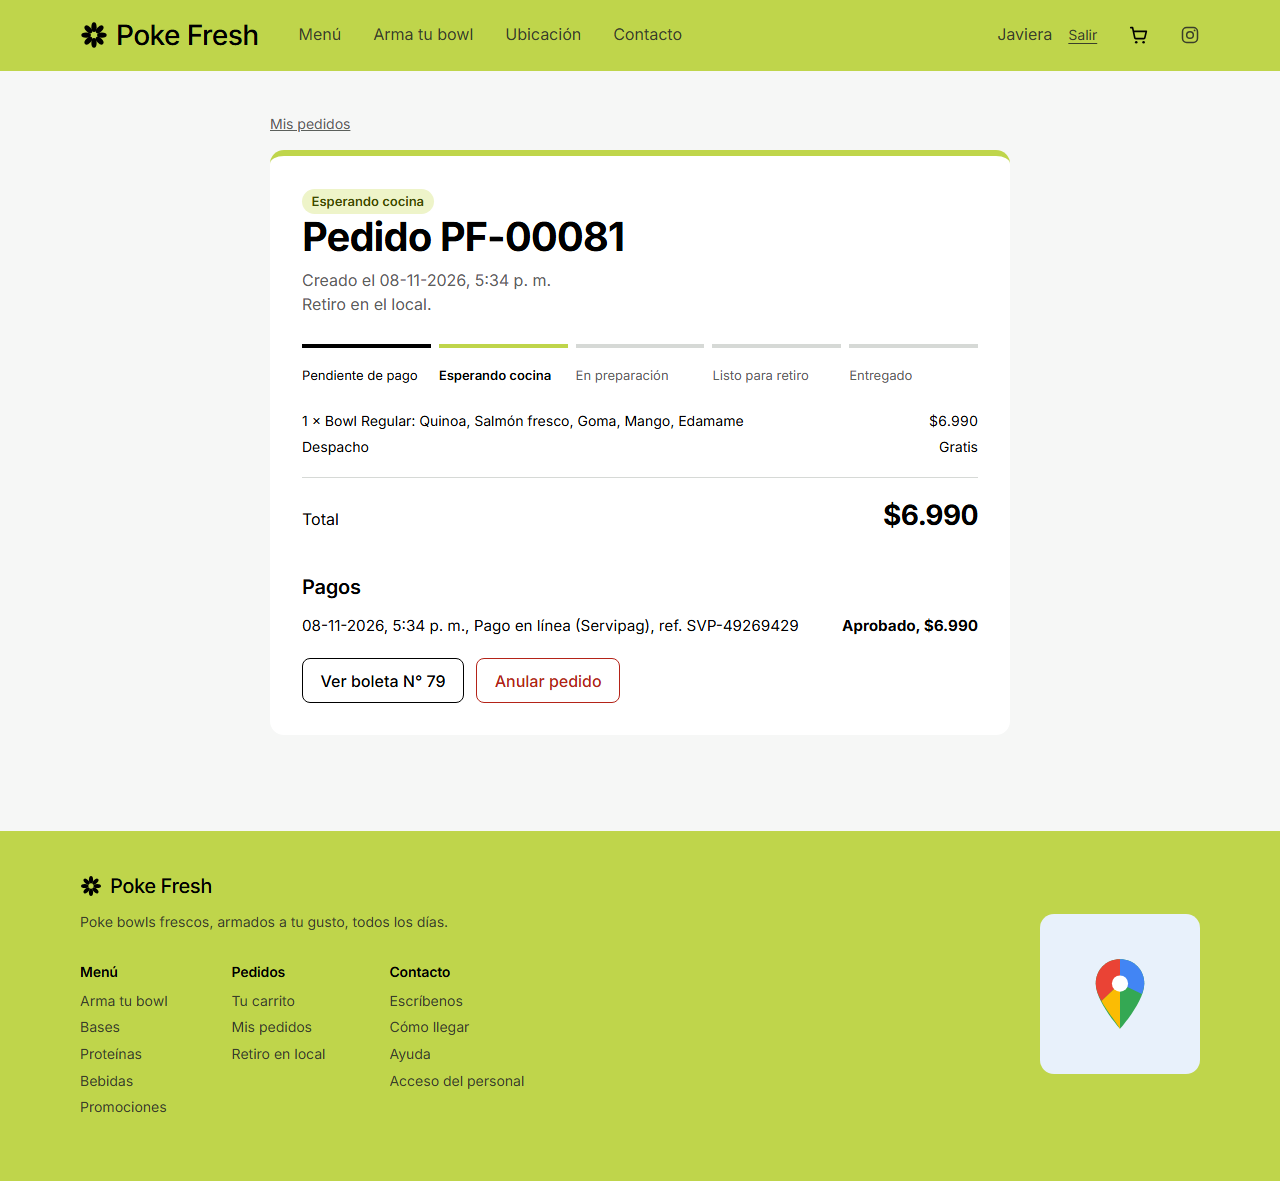
\includegraphics[width=\linewidth,height=0.85\textheight,keepaspectratio]{../evidencias/pantallas/06-pedido-pagado-graphql.png}
\caption{Pantalla del pedido (06-pedido-pagado-graphql.png): el pedido, servicio de pedidos, junto a la sección “Pagos”, servicio de pagos, obtenidos con resumenPedido}
\end{figure}

\begin{figure}[H]
\centering
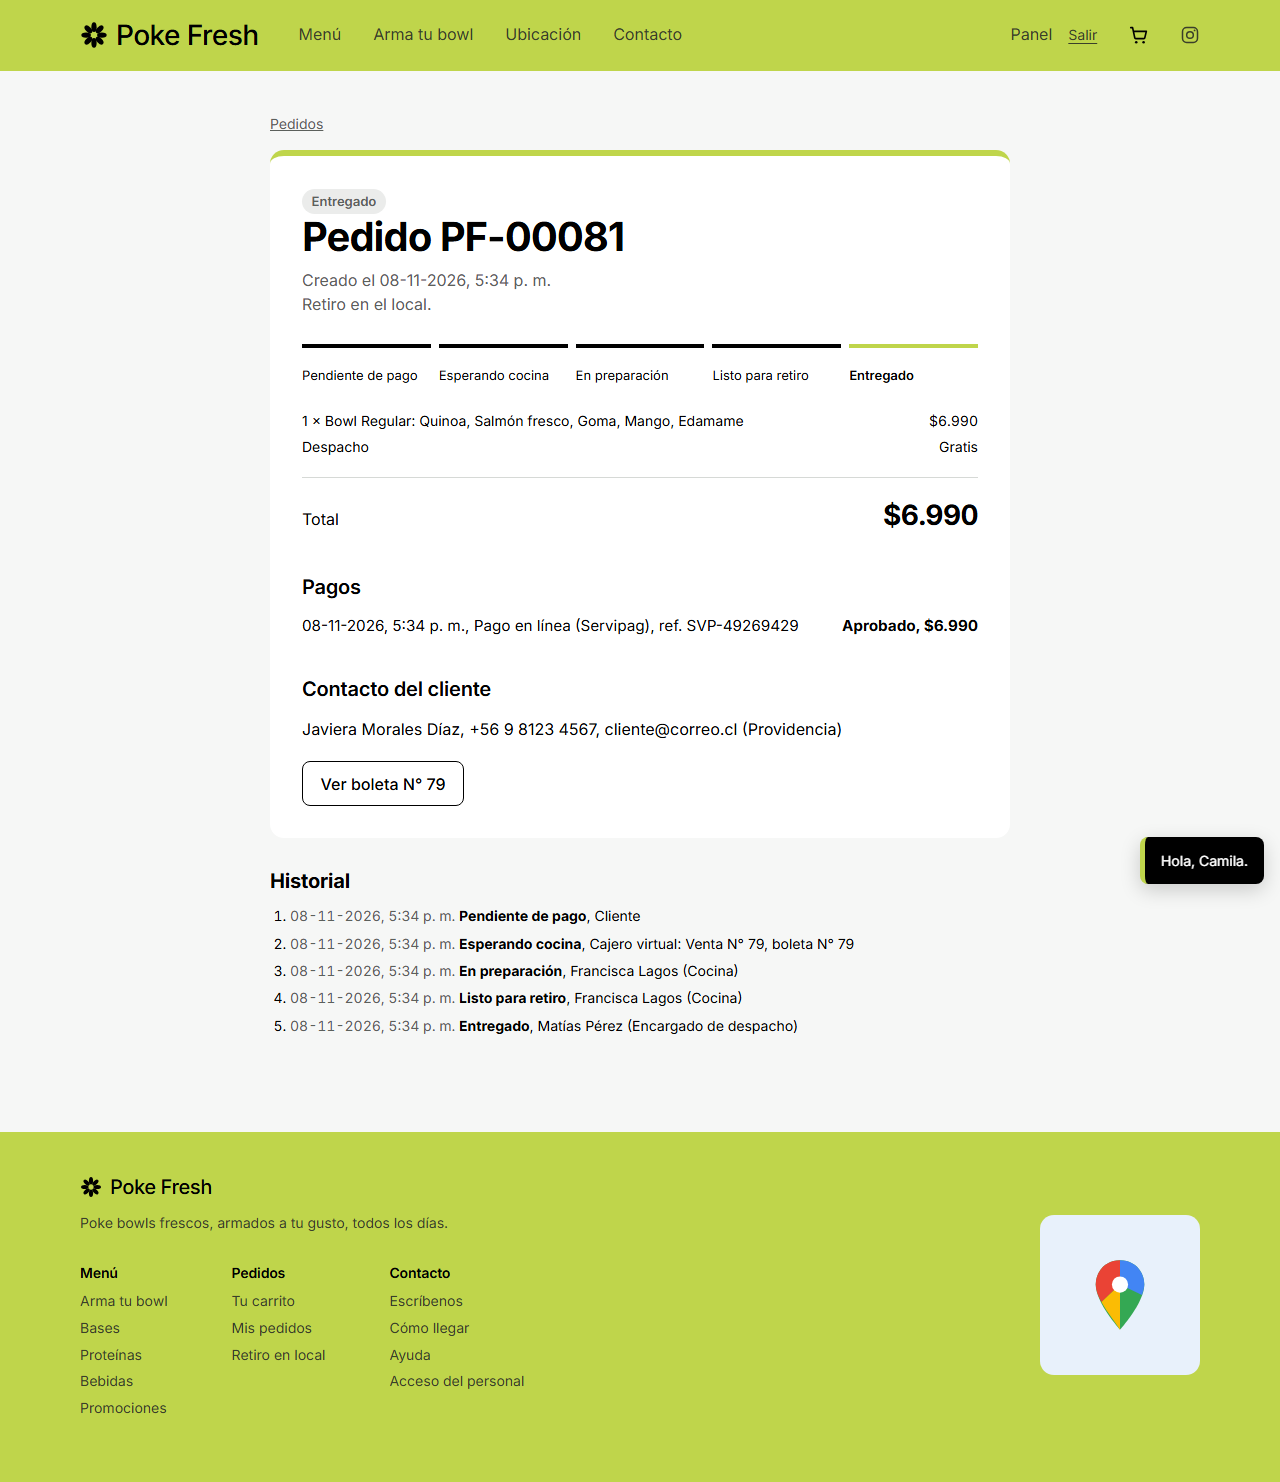
\includegraphics[width=\linewidth,height=0.85\textheight,keepaspectratio]{../evidencias/pantallas/14-pedido-vista-admin.png}
\caption{Vista del administrador (14-pedido-vista-admin.png): además aparece “Contacto del cliente”, servicio de clientes, solo para admin}
\end{figure}

\begin{figure}[H]
\centering
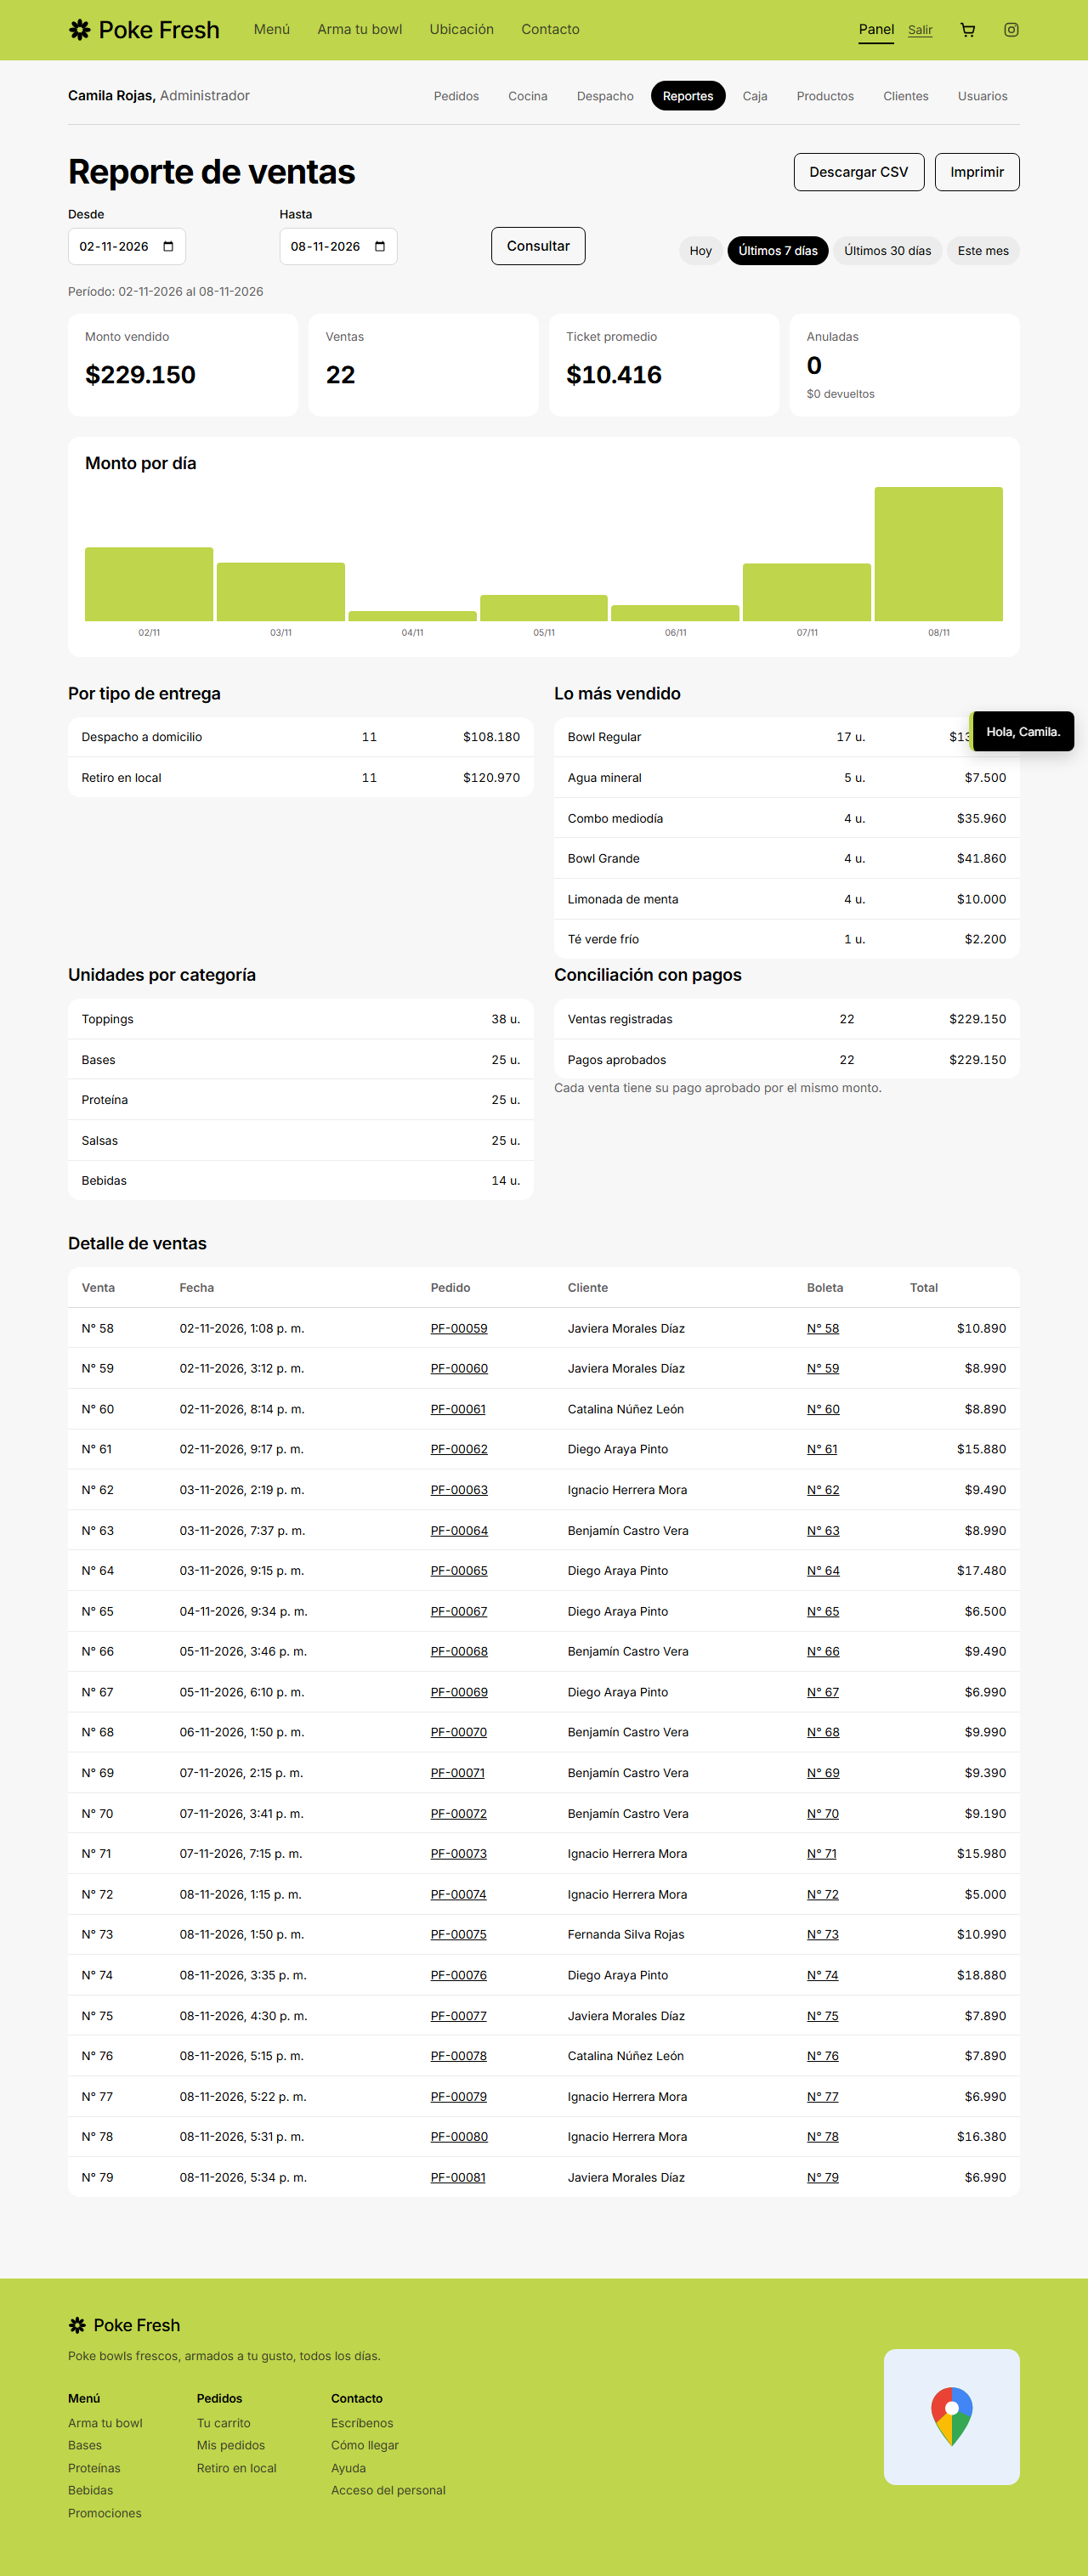
\includegraphics[width=\linewidth,height=0.85\textheight,keepaspectratio]{../evidencias/pantallas/11-reportes-graphql.png}
\caption{Reportes (11-reportes-graphql.png): “Unidades por categoría” y “Conciliación con pagos”, desde reporteVentas}
\end{figure}

\texttt{recorrido.\allowbreak{}json} lista las rutas de la API que usó el navegador: todas bajo \texttt{/\allowbreak{}api/\allowbreak{}v1}; ninguna a un servicio interno.


\textbf{Qué comprobamos.} Que la consulta junta de verdad datos de tres o cuatro servicios; que cada servicio mantiene su autoridad (la propiedad del pedido la decide pedidos); que pedir campos de más no filtra datos restringidos (si un cliente pide \texttt{cliente \{ email \}}, recibe PROHIBIDO); y que la red privada y los permisos funcionan con el sistema en marcha (casos 7.5, 7.9 y 8.1 a 8.3).

